\section{Continuous Occlusion Model}
\label{sec:setup}


%We want to solve the problem of segmenting point tracks into object so that the consensus of points can be used draw inferences about the object. In particular given a set of correspondence points on consecutive frames $(\trackpj{t}, \trackpj{t-1})$, object localizations $\relp{i}{t}$ and object dimensions $\dimsn{i}$ we want to figure out which points belong to which object. We call this the association problem. Even if the pose of the object is not immediately available we propose the use of hypothesized pose of the object as we show in the localization estimation experiments. 

\def\TP{TP}
A common parametric modeling for objects, especially traffic participants (TP) in road scene understanding, is as opaque cuboids.\footnote{Notable exceptions exist, such as \cite{Zia_etal_2014}, but we note that such models are expensive, application-specific and still discontinuous.} However such models introduce discontinuities in the problem formulation and do not adequately account for uncertainties in pose and dimensions. With this motivation, we introduce our representation of 3D objects and our modeling of object-object relationships, which lead to a continuous occlusion model that correctly accounts for uncertainties in position and dimensions. We refer the reader to Figure~\ref{fig:reflectiontransimission} for an illustration of the proposed concepts.

%In this section, we introduce our representation of 3D objects and our modeling of object-object occlusion relationships. We refer the reader to Figure~\ref{fig:reflectiontransimission} for an illustration of the proposed concepts.

\begin{figure}
  \usetikzlibrary{calc}
  \centering
  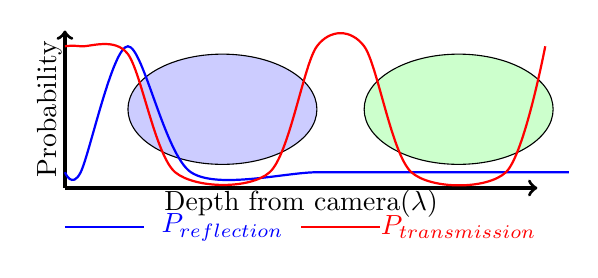
\begin{tikzpicture}
         \path [fill=blue!20,draw] (0,0) ellipse (1.2 and 0.7);
     \path [fill=green!20,draw] (3,0) ellipse (1.2 and 0.7);
     \coordinate (o) at (-2,-1);
     \draw(o) edge [->,very thick] node (xa) {} +(6, 0);
     \node at ($(xa) + (0, -0.2)$) {Depth from camera($\lambda$)};
     \draw(o) edge [->,very thick] node (ya) {} +(0, 2);
     \node [rotate=90]at ($(ya) + (-0.2, 0)$) {Probability};
    \draw [thick,blue]plot [smooth] coordinates {($(o)+(0,0.2)$) ($(o)+(0.2,0.2)$) ($(o) + (0.8, 1.8)$) ($(o)+(1.6,0.2)$) ($(o)+(3.2,0.2)$) 
      %($(o)+(3.8,1.8)$)  % Transmission prob corresponds to particular object
    ($(o)+(4.4,0.2)$) ($(o)+(6.4,0.2)$) };
    \draw [thick,red] plot [smooth] coordinates {($(o)+(0,1.8)$) ($(o)+(0.2,1.8)$) ($(o) + (0.8, 1.7)$) ($(o)+(1.4,0.2)$) ($(o)+(2.6,0.2)$) ($(o)+(3.2,1.8)$) ($(o)+(3.8,1.8)$) ($(o)+(4.4,0.2)$) ($(o)+(5.6,0.2)$) ($(o)+(6.1,1.8)$) };
   \draw [thick, blue] ($(o) + (0,-0.5)$) -- +(1,0) +(2,0) node {$P_{\text{reflection}}$};
   \draw [thick, red] ($(o) + (3,-0.5)$) -- +(1,0) +(2,0) node {$P_{\text{transmission}}$};

  \end{tikzpicture}
  \vspace{-0.3cm}
  \caption{\small We represent objects as translucent ellipsoids which allows formulation of transmision and reflection probabilities. This figure shows the reflection probability for the first object (violet) which is highest closer to the camera. Also note that the transmission probability is inversely proportional to occupancy.}
  \label{fig:reflectiontransimission}
  \vspace{-0.3cm}
\end{figure}

\vspace{-0.3cm}
\paragraph{Occupancy model for traffic participants}
Intuitively, we consider traffic participants to be regions of 3D space with a high probability of occupancy. We model the uncertainty in occupancy as a translucency function, with regions more likely to be occupied by an object considered more opaque, while regions more likely to be free space are more transparent. Based on this intuition, we model objects as translucent 3D ellipsoids whose opacity is maximum at the center and falls off towards the edges. In particular, we model the occupancy at 3D location $\bx$ corresponding to an object $O_i$ centered at $\bp_i$ as:
\begin{align}
  f^i_{\text{occ}}(\bx) = \cL(\bx; \bp_i, \bSigma_i)
\end{align}
where $\cL(\cdot)$ is the logistic function given by
\begin{align}
  \cL(\bx; \bp, \bSigma) = \frac{1}{1 + e^{-k(1 - d(\mathbf{x},\bp))}},
\end{align}
with $d(\bx, \bp) = (\bx-\bp)^\top\bSigma(\bx-\bp)$ being the Mahalanobis distance. We set $k = 10\ln{49}$ as the value that allows the logistic function $\cL$ to drop to $0.98$ at a distance $d = 0.9$ from the object center. The spread of the ellipsoid, determined by $\bSigma_i$, depends of the dimensions of the object. Please refer to the supplementary material for the computation of $\bSigma_i$ from object dimensions.


\vspace{-0.3cm}
\paragraph{Image formation}
Given the above occupancy representation of the scene, a point on an object is observed in the camera when precisely two conditions are satisfied. First, the backprojected ray from the observed image pixel is transmitted through free space until it reaches the object. Second, the ray encounters an opaque enough object surface and is reflected. More formally, the probability of observation of a point $\bx_j$ on object $O_i$ is given by
\begin{align}
P^{ij}_{\textit{observation}} = P^{ij}_{\textit{reflection}}P^{j}_{\textit{transmission}}.
\label{eq:imgform}
\end{align}
The reflection probability ensures the presence of an object to constitute the observation, while the transmission probability allows us to model occlusions. The forms of these two functions are described next.


\vspace{-0.3cm}
\paragraph{Reflection probability}
Consider a 3D point $\bx_j$ observed in the image at pixel $\bu_j$. Let $\bK$ be the intrinsic calibration matrix for the camera and $\ray = \displaystyle\frac{\bK^{-1}\bu_j}{\lVert \bK^{-1}\bu_j \rVert}$ be the unit vector along the backprojected ray from the camera center passing through $\bu_j$. Then, the probability of reflection at depth $\lambda$ along the ray $\ray$, by an object $O_i$, is determined by the gradient of the object's occupancy function $f_{occ}^i$:
\begin{align}
  P^{ij}_{\textit{reflection}} (\lambda) = (\max \{0, \nabla {f^i_{occ}}(\bx_j)^\top \ray \})^2
\label{eq:evalPrefl}
\end{align}
The $\max \{ \}$ ensures that the negative probability due to gradient in the direction opposite to the ray is clipped off and squaring the function allows it to be smooth near zero. We note that in the extreme case of an object being Lambertian, the above reverts to a (squared) Lambertian reflection.


\vspace{-0.3cm}
\paragraph{Transmission probability}
\label{sec:ptransmission}
Since we are modeling occupancy as transparency, we derive inspiration from optics for the modeling of translucent objects. A model for transmission of light across a distance $\alpha$, through a medium of density $\rho$ and opacity $\beta$ is given by the Beer-Lambert Law:
\begin{align}
I(\alpha) = I_0 e^{-\beta\rho\alpha}.
\end{align}
%
In our formulation of scene occupancy, both opacity and density at a scene point $\bx_j$ are encapsulated within the total occupancy function summer over all objects, $\occftot = \sum_i \occf$. Further, the domain of our ocupancy function $\occftot$ is $[0, 1]$ instead of $[0, \infty)$ for opacity $\beta$. Thus, we replace $e^{-\beta\rho}$ by the transparency function $1 - \occftot$ and consequently, the transmission probability over a small distance $d\lambda$ is given by
%
\begin{align}
  \!\!\!\! P^j_{\textit{transmission}}(\lambda + d\lambda) = P^j_{\textit{transmission}}(\lambda) (1-\occftot)^{d\lambda}.
\end{align}
%
Thus, for an image point $\bu_j$ to correspond to a 3D point $\bx_j$ at depth $\lambda$ along the backprojected ray $\ray$, the ray must be transmitted through space with the probability
\begin{align}
P^j_{\textit{transmission}}(\lambda) = \prod_{c}^{\lambda} (1 - \occft{\lambda \ray})^{d\lambda}.
\label{eq:ptrans-integral}
\end{align}
Here, $\prod_{c}^{\lambda}$ represents a \emph{product integral} from $c$ to $\lambda$, where $c$ is the position of camera screen, considered here to be equivalent to the focal length of the camera .\footnote{A product integral is a simple integral in the log domain: 
\vspace{-0.2cm}
\begin{equation}
\prod_{c}^{\lambda} (1 - f_{occ}(\lambda \ray))^{d\lambda} = e^{\int_{c}^{\lambda} \ln{(1 - f_{occ}(\lambda \ray))}{d\lambda}}. \nonumber
\end{equation}
}

In practice, the integral for transmission probability \eqref{eq:ptrans-integral} is difficult to compute even numerically. So we choose a parameterization in the form of a product of sigmoid functions, which is a reasonable approximation to the behaviour of the transmission probability:
%
\newcommand{\Ptransmission}{P_{\textit{transmission}}}%
\begin{align}
  \Ptransmission^j(\lambda) = \prod_i (1 - \cL_u (\bu; \bmu_i, \bGamma_i) \cL_{\lambda}(\lambda; \meandepth{i})),
\label{eq:evalCumulativePtrans}
\end{align}
%
where $\cL_u(.)$ is sigmoid in image domain, with $\bmu_i$ and $\bGamma_i$ representing the elliptical projection of object $O_i$ in the image and $\cL_{\lambda}(.)$ is sigmoid in the depth domain with $\meandepth{i}$ the mean depth of object $O_i$. That is,
%
\begin{align}
\cL_u(\bu; \bmu_i, \bGamma_i) &= \frac{1}{1 + e^{-k_u(1 - (\bu - \bmu_i)^\top \bGamma_i (\bu - \bmu_i))}} \\
  \cL_{\lambda}(\lambda; \meandepth{i}) &= \frac{1}{1 + e^{-k_d(\lambda - \meandepth{i})}}
\end{align}
%
In Figure \ref{fig:compare:exact:approx:ptrans}, we compare the exact and relative formulations of transmission probability given by \eqref{eq:ptrans-integral} and \eqref{eq:evalCumulativePtrans}, respectively. Note that the choice of mean depth of the object causes some deviation from the exact transmission probability. However, the shift of transmission probability anywhere through the object is still a reasonable approximation as occluded points can only lie outside the object. On the other hand, it yields significant computational savings since ray intersections with an ellipsoid are expensive to evaluate densely.

%the computation of ray intersection with ellipsoid is expensive to compute for every ray and the shift of transmission probability anywhere through the object is a reasonable approximation as the occluded points can only lie outside the object.

\begin{figure}
\centering
  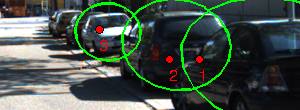
\includegraphics[width=0.9\columnwidth]{results/plotPtransmission_exact_vs_approx_pt_vis-small.png}\\
  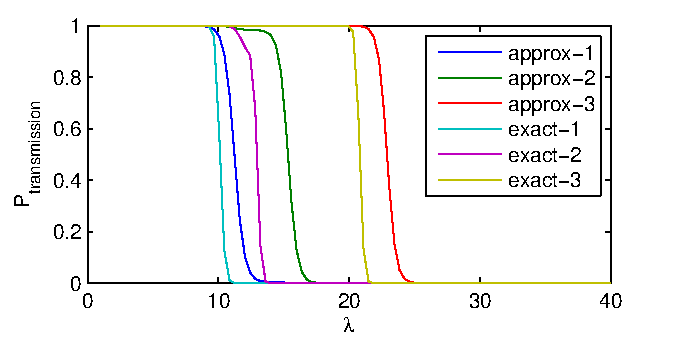
\includegraphics[trim=0.0 0 0.3in 0, clip, width=0.9\columnwidth]{results/plotPtransmission_exact_vs_approx.pdf}
  \vspace{-0.3cm}
  \caption{\small Comparing the approximate $\Ptrans$ with exact version. The drop in approximate version of $\Ptrans$ is delayed because we assume drop at the center of the car rather than camera facing face of the car.}
  \label{fig:compare:exact:approx:ptrans}
  \vspace{-0.3cm}
\end{figure}

Thus, we have modeled the transmission probability to effectively capture the effect of occlusion due to all traffic participants in a scene that lie along a particular ray. We reiterate that our reflection and transmission probabilities are continuous functions, which allows us to keep the problem formulation in the continuous domain.
% allowing for easier optimization.
